\documentclass[paper=a4,10pt]{scrartcl}

\usepackage[utf8x]{inputenc}
\usepackage[ngerman]{babel}
\usepackage[T1]{fontenc}

\usepackage{graphicx}
\usepackage{float}
\usepackage{subcaption}

\usepackage{fancyref}

\usepackage[numbers,square,sort]{natbib} %praktikumsquellenvorgabe
\usepackage{amsmath}
\usepackage{amssymb}

\usepackage{url}
\usepackage{hyperref}

\usepackage[a4paper, includehead, includefoot]{geometry}
\geometry{left=2cm, right=2cm, top=2cm, bottom=2cm}

%\usepackage{multibib}
%\\bibliographystyle{unsrt}


\title{Fouriertransformation-Notizen}
%\author{Robert Kummer}
%\date{2019}

\begin{document}
\pagenumbering{gobble}
\maketitle
\newpage
\tableofcontents
\newpage
\pagenumbering{arabic}
\setcounter{page}{1}

\section{Sinus plus Sinus}
% der Link ist sehr usefull https://www.youtube.com/watch?v=G7djzoTRaic
Wenn man eine Sinusähnliche Welle mit einer anderen addiert, erhält man erneut eine Sinusförmige Welle. Das lässt sich über ein Zeigerdiagramm veranschaulichen. \\
\noindent
Als Beispiel will ich die folgende Summe berechnen:
\begin{align}
	A \cos(\omega x) + B \sin(\omega x)
\end{align}
In diesem Bsp haben beide Wellen unterschiedliche Amplituden, aber die selbe Frequenz und die selbe Phase, nämlich Null. Zur Verdeutlichung die Abb. \ref{fig:sps}. In schwarz soll der Sinus dargestellt sein und er startet bei $x=B$ In dem Bild ist jetzt $\omega x$ als $\omega t$ geschrieben. Wenn jetzt ein beliebiger Punkt in der Zeit, (oder in x) erreicht ist, dann steht der Sinus ja irgendwo und das soll hier oBdA zum Zeitpunkt des schwarzen Vektors sein. Der Cosinus ist in orange dargestellt und da er einfach nur ein um $\frac{\pi}{2}$ verschobener Sinus ist ($\cos(\omega t) = \sin(\omega t + \frac{\pi}{2})$), ist er hier auch so dargestellt (unter der Annahme, dass A kleiner als B ist).
\begin{figure}[H]
	\centering
	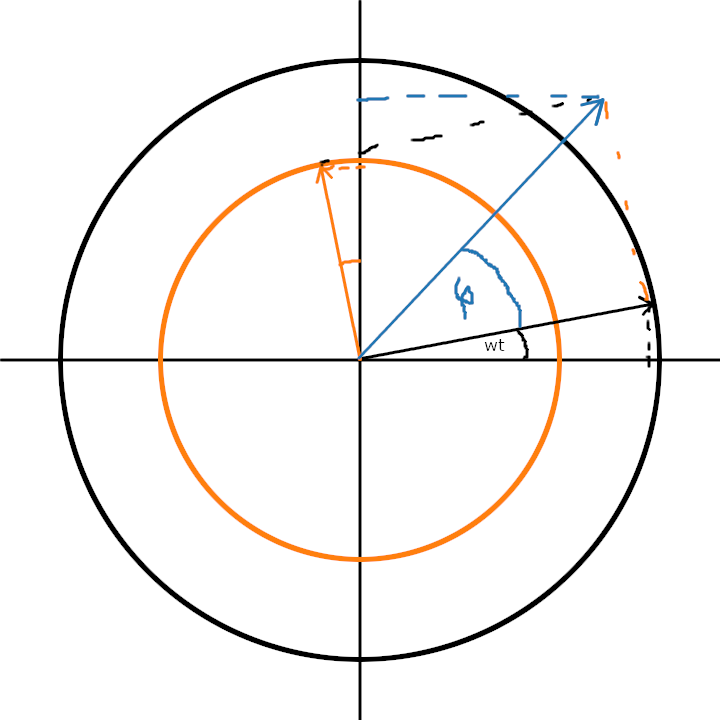
\includegraphics[width=0.4\textwidth]{./bilder/sinus_plus_sinus.png}
	\caption{Veranschaulichung}
	\label{fig:sps}
\end{figure}
\noindent
Jetzt will man ja die Summe beider Sinusfunktionen haben. Das kann man machen, indem man die jeweiligen y-Komponenten der Vektoren zum gegebenen Zeitpunkt addiert. Es werden einfach direkt beide Vektoren addiert und es kommt der blaue Vektor raus, dessen y-Komponente der Summer der Sinusse entspricht. Wenn man das jetzt zu jeder Zeit macht, dreht sich der blaue Vektor mit der selben Frequenz wie die anderen beiden und seine y-Komponente enspricht immer der Summe der Sinusse. \\
\noindent
Der entscheidende Gedanke ist jetzt: Das ist eine eigene Sinusschwingung! Die Amplitude davon ergibt sich über den Pythagoras. Man muss noch beachten, dass der neue Sinus mit einer Phase $\phi$ beginnt zu schwingen und die ergibt sich über $\tan^{-1}(\frac{A}{B})$. Das Ergebnis sieht also so aus:
\begin{align}
\sqrt{A^2 + B^2} \sin \left(\omega t + \tan^{-1}\left( \frac{A}{B} \right) \right) = C \sin(\omega t + \phi)
\end{align}
Wenn die Ausgangssinusse noch Phasen haben, dann ist die Herangehensweise die selbe, es kommen nur noch ein paar Ausdrücke dazu, weil man die eben mit berücksichtigen muss.




\end{document}